%\documentclass[sigconf, titlepage, twoside]{acmart}
\documentclass[12pt,titlepage, twoside]{article}
%\usepackage{titlesec}

% language stuff
\usepackage{german}           % deutsche Überschriften etc.
\usepackage{ziffer}           % For , instead of . as Decimal Separator
\usepackage[utf8]{inputenc} % direkte Eingabe von Umlauten

% Layout-Einstellungen
\usepackage{parskip}          % Abstand statt Einrückung
\frenchspacing                % no extra space after periods
\usepackage{parskip}          % paragraph gaps instead of indentation
\usepackage{times}            % default font Times
\tolerance=9000               % avoid words across right border

% miscellaneous
\usepackage{graphicx}         % graphics
\usepackage{subcaption}       % subfigures
\usepackage{hhline}           % double lines in tables
\usepackage{amsfonts}         % real numbers etc.
\usepackage[rightcaption]{sidecap} % figure captions on the right (optional)
\usepackage{hyperref}         % for URLs
\usepackage{listings}         % for code samples
\usepackage{fancyhdr}         % for header line
\usepackage{lastpage}         % for last page count

\usepackage{makecell}

\usepackage{xcolor}           % Code highligting

\usepackage{amsmath}

\colorlet{punct}{red!60!black}
\definecolor{background}{HTML}{EEEEEE}
\definecolor{delim}{RGB}{20,105,176}
\definecolor{string}{RGB}{0,0,255}
\colorlet{numb}{magenta!60!black}

\lstdefinelanguage{json}{
    basicstyle=\normalfont\ttfamily,
    %numbers=left,
    %numberstyle=\scriptsize,
    stepnumber=1,
    numbersep=8pt,
    showstringspaces=false,
    breaklines=true,
    frame=lines,
    stringstyle=\ttfamily\color{string},
    %backgroundcolor=\color{background},
    literate=
     *{0}{{{\color{numb}0}}}{1}
      {1}{{{\color{numb}1}}}{1}
      {2}{{{\color{numb}2}}}{1}
      {3}{{{\color{numb}3}}}{1}
      {4}{{{\color{numb}4}}}{1}
      {5}{{{\color{numb}5}}}{1}
      {6}{{{\color{numb}6}}}{1}
      {7}{{{\color{numb}7}}}{1}
      {8}{{{\color{numb}8}}}{1}
      {9}{{{\color{numb}9}}}{1}
      {:}{{{\color{punct}{:}}}}{1}
      {,}{{{\color{punct}{,}}}}{1}
      {\{}{{{\color{delim}{\{}}}}{1}
      {\}}{{{\color{delim}{\}}}}}{1}
      {[}{{{\color{delim}{[}}}}{1}
      {]}{{{\color{delim}{]}}}}{1},
}
%
%\newcommand{\imageSizeTwo}{0.49\textwidth}
%\newcommand{\imageSizeTwoHeight}{7.5cm}
\newcommand{\imageSizeTwo}{0.35\textwidth}
\newcommand{\imageSizeTwoHeight}{4.5cm}
\newcommand{\imageSizeThree}{0.3\textwidth}
\newcommand{\imageSizeThreeHeight}{5cm}
\newcommand{\imageWidthFour}{width=2cm height=2cm}

% Hier bei Bedarf die Seitenränder einstellen
\usepackage{geometry}
%\geometry{a4paper}
\geometry{a4paper, top=3.5cm, bottom=2.5cm} 

% Kopf- und Fußzeile
\fancyhead{} % clear all header fields
\fancyhead[RO,LE]{\leftmark}

%%%%%%%%%%%%%%%%%%%%%%%%%%%%%%%%%%%%%%%%%%%%%%%%%%%%%%%%%%%%%%
\begin{document}

\section{Stand der Technik}
%-------------------------------------------------------------
\label{sec:stand}

SIFT \cite{Sift} ist der wohl bekannteste Ansatz und wird häufig als Goldstandard verwendet, um Verfahren miteinander zu vergleichen. SIFT hat allerdings den Nachteil, dass es zu langsam für Echtzeitanwendungen ist.
SIFT ermittelt die Kandidaten-Punkte im Kern mittels des Difference of Gaussians Verfahrens (DoG), welches aus drei Schritten besteht. Im ersten Schritt wird auf das Bild in verschieden starken Stufen ein Weichzeichner (diskreter Gauß-Filter) angewandt.
Damit liegt das Bild mit zunehmend niedrigerem Kontrast vor. Zwischen den einzelnen Kontraststufen wird die Differenz ermittelt. Liegen die Differenzen vor, kann nach Extrempunkten in den Differenzen gesucht werden.
Hierbei wird jedes Pixel im Bild mit seinen direkten Nachbarn und denen in der vorherigen und nachfolgenden Stufe verglichen. Ist das Pixel ein Extrempunkt, wird es als Kandidat gewählt.
DoG wird auf mehreren Skalierungen des Bildes angewandt, um Skalierungs-Invarianz zu erreichen.
Im Anschluss werden die Kandidaten gefiltert. Kandidaten, die einen niedrigen Intensitätswert haben oder eine Kante darstellen, werden hierbei ausgeschlossen.
Sind die Positionen der Features bekannt, kann der Feature-Vektor $f$ für den Punkt $p$ ermittelt werden. 
Um den Deskriptor für den Punkt $p$ zu berechnen werden zwei Größen benötigt. Zum einen die Skalierung, in der der Punkt ermittelt wurde - diese ist bereits bekannt - und zum anderen die Orientierung des Punktes.
Um diese zu bestimmen werden in einem Bereich um den Punkt $p$ die Gradienten berechnet und in ein Histogramm abgetragen. Der Histogramm-Eintrag (Bin) mit dem größten Wert entscheidet die Orientierung des Punktes.
Sind Skalierung und Orientierung bekannt, wird auf Basis der beiden ein Bereich gewählt und in einen $16\times 16$ großen Bereich skaliert. 
Dieser Bereich wird in $16$ gleichgroße Bereiche unterteilt, für die jeweils ein Histogramm gebildet wird. 
Die Bins der Histogramme beschreiben in $8$ diskreten Stufen die Orientierung der Punkte im jeweiligen Bereich. 
Die einzelnen Punkte tragen die Stärke des Gradienten im jeweiligen Bin des Histogramms ab.
Diese Histogramme bilden den Feature-Vektor $f$, der für den Vergleich genutzt wird.

SURF \cite{SURF} ist ähnlich aufgebaut wie SIFT, nur wird der genutzte Gauß-Filter durch Box-Filter, die besonders effizient berechnet werden, approximiert.
Des Weiteren wird der Feature-Vektor anders gebildet. Mit beiden Anpassungen wird eine bessere Leistung erreicht.
Bei der Approximation des Gauß-Filters wird zuerst das Integral-Bild $I_\Sigma$ (Gleichung \ref{eq:sfm:surf:integral}) aus den Intensitätswerten $I$ des Bildes berechnet.
\begin{equation}
    \label{eq:sfm:surf:integral}
    I_\Sigma (x,y) = \sum_{i=0}^{i\leq x}\sum_{j=0}^{j\leq y}I(i,j)
\end{equation}
Ist $I_\Sigma$ bekannt, kann die Intensitäts-Summe eines beliebigen rechteckigen Ausschnitts sehr effizient berechnet werden. 
Hierzu werden nur die Werte aus $I_\Sigma$ für die Eckpunkte $P_1$ - $P_4$ eines Ausschnittes $D$ benötigt.
Die Fläche für $D$ lässt sich dann mit $f(D)$ (Gleichung \ref{eq:sfm:surf:f}) effizient berechnen.
\begin{equation}
    \label{eq:sfm:surf:f}
    f(D) = I_\Sigma(x_{P_1}, y_{P_1}) + I_\Sigma(x_{P_4}, y_{P_4}) - I_\Sigma(x_{P_2}, y_{P_2}) - I_\Sigma(x_{P_3}, y_{P_3})
\end{equation}
Um den Gauß-Filter mit Box-Filtern zu approximieren, wird die Determinante der Hesse-Matrix genutzt. 
Um die approximierte Hesse-Matrix für einen Punkt $p$ mit der Skalierung $s$ zu bilden, muss man die zweite Ableitung der Gauß-Funktion nach $x$, $y$ und $xy$ mit Box-Filtern approximieren (Siehe Gleichung \ref{eq:sfm:surf:h}).
\begin{equation}
    \label{eq:sfm:surf:h}
    H_{approx.}(p,s) = \left( \begin{smallmatrix} D_{xx}(p,s)&D_{xy}(p,s)\\ D_{xy}(p,s)&D_{yy}(p,s) \end{smallmatrix} \right)
\end{equation}
Die Determinante der Hesse-Matrix kann dann wie in Gleichung \ref{eq:sfm:surf:det} berechnet werden, wobei $w\approx 0,9$ ist und den Fehler der Approximation minimieren soll.
\begin{equation}
    \label{eq:sfm:surf:det}
    det(H_{approx.}) = D_{xx}D_{yy}-(wD_{xy})^2
\end{equation}
Ein Beispiel für die Box-Filter ist in Abbildung \ref{fig:surf:filter} zu sehen. Sowohl die verschiedenen Gauß-Stufen als auch die verschiedenen Skalierungs-Stufen werden durch ein Vergrößern der Filter-Maske erreicht.
\begin{figure}
    \centering
    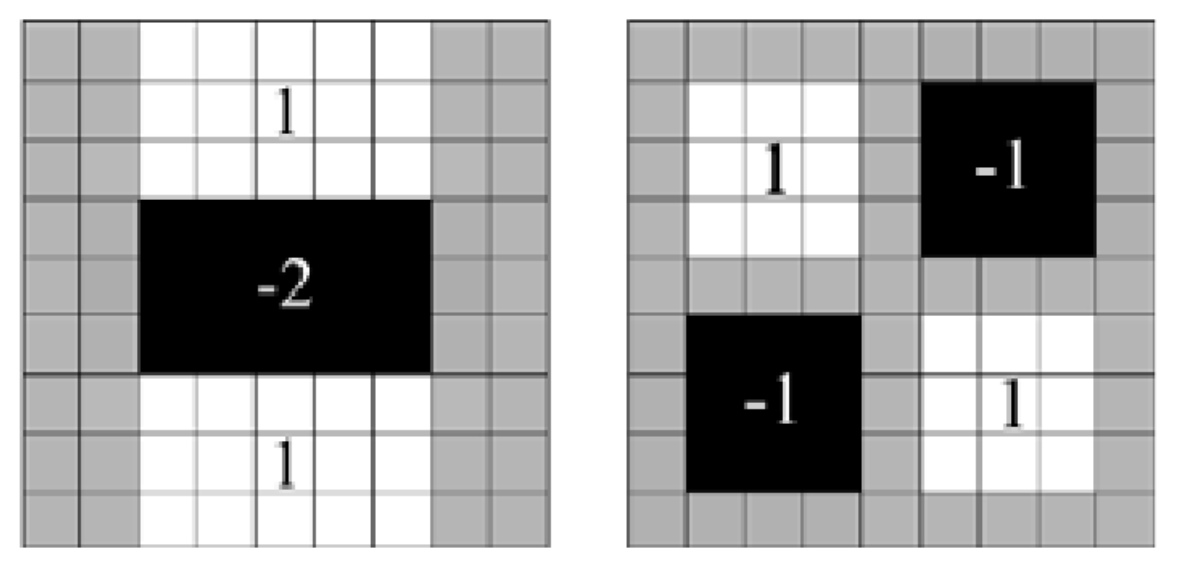
\includegraphics[width=0.5\textwidth]{./Images/SURF_BoxFilter.png}
    \caption{Box-Filter für zweite Ableitung nach y (links) und Ableitung nach xy (rechts). \cite{SURF}}
    \label{fig:surf:filter}
\end{figure}
Der Deskriptor wird in zwei Schritten berechnet. Zuerst wird die Hauptorientierung des Punktes berechnet. Dann wird auf dieser und der Skalierung basierend ein Bereich in dem Bild gewählt und in 16 Bereiche unterteilt.
Für jeden der 16 Bereiche wird die Intensität der Punkte in einem $4$ Bin großen Histogramm abgetragen, was zu einem Feature-Vektor der Größe $64$ führt.

ORB \cite{ORB} geht diesen Nachteil an, indem zuerst das Massezentrum des Bildes $C$ (Gleichung \ref{eq:sfm:orb:c}) und dessen Orientierung $\theta$ (Gleichung \ref{eq:sfm:orb:theta} )
über die Momente $m_{00}$, $m_{10}$ und $m_{01}$ (Gleichung \ref{eq:sfm:orb:m}) berechnet wird.
Mit diesen Parametern werden die Koordinaten der Paare umgeformt, um so der Anfälligkeit für Rotation entgegen zu wirken. 
Des Weiteren liefert ORB eine gelernte Paar-Auswahl von $256$ Paaren, die dahingehend optimiert ist, dass die Paare unkorreliert sind und eine hohe Varianz aufweisen.

\begin{equation}
    \label{eq:sfm:orb:m}
    m_{pq} = \sum_{x,y}{x^py^qI(x,y)}
\end{equation}
\begin{equation}
    \label{eq:sfm:orb:c}
    C = ( \frac{m_{10}}{m_{00}}, \frac{m_{01}}{m_{00}} )
\end{equation}

\begin{equation}
    \label{eq:sfm:orb:theta}
    \theta = atan2(m_{01},m_{10})
\end{equation}

Um aus den korrespondierenden Bildpaaren auf die Positionen der Kameras zu schließen, wird die Fundamental-Matrix $F=K_1^{-1T}EK_2^{-1}$ für jedes Bildpaar ermittelt. 
$K_1$ und $K_2$ sind die beiden Kalibrierungs-Matrizen der Kameras und $E$ ist die Essential-Matrix, welche die Bewegung und Rotation der Kamera beschreibt.
Ist die Kalibrierung der Kamera bekannt, kann direkt $E$ berechnet werden.
$F$ beschreibt die Kamera-Bewegung und Rotation von einem zum anderen Bild, hat den Rang $2$ und bezieht dabei die Kalibrierung der Kameras mit ein.
%$E$ kodiert die Transformation bestehend aus der Rotation $R$ und der Translation $t$ zwischen den beiden Kamera-Positionen.
Um $F$ zu ermitteln werden mindestens acht korrespondierende Features $(p_{A1},p_{B1})...(p_{A8},p_{B8})$ zwischen den Bildern $A$ und $B$ eines Paares benötigt. 
Die Bildpunkte $p_{Ai}$ und $p_{Bi}$ der Paare sind dabei nicht in Pixel-Koordinaten, sondern relativ zum Bild-Ebenen-Zentrum angegeben. 
Die Koordinaten liegen also im Bereich  $[-1, 1]$.
Da es sich um homogene Koordinaten handelt, wird neben dem $x$ und $y$ Wert noch eine Eins hinzugefügt.
Hierzu werden mindestens acht Gleichungen der Form $p_{Ai}^TFp_{Bi}=0$ (Siehe auch Gleichung \ref{eq:sfm:ax:line}) gebildet und daraus ein Gleichungssystem der Form $Af=0$ erzeugt, wobei $f$ die Unbekannten aus $F$ enthält.
\begin{equation}
    \label{eq:sfm:ax:line}
    \begin{aligned}
    x_{p_{Ai}}x_{p_{Bi}}f_1 + x_{p_{Ai}}y_{p_{Bi}}f_2 + x_{p_{Ai}}f_3 + &\\
    y_{p_{Ai}}x_{p_{Bi}}f_4 + y_{p_{Ai}}y_{p_{Bi}}f_5 + y_{p_{Ai}}f_6 + &\\
    x_{p_{Bi}}f_7 + y_{p_{Bi}}f_8 + f9 &= 0
    \end{aligned}
\end{equation}
Das Gleichungssystem wird mittels Singulärwertzerlegung (SVD) gelöst. Man erhält drei Matrizen $U$, $S$ und $V$. $U$ hat die Größe $m\times m$, $S$ die Größe $m\times 9$ und $V$ die Größe $9\times 9$.
$S$ ist eine Diagonal-Matrix, deren Einträge die Singulärwerte von $A$ in absteigender Reihenfolge enthalten.
Aus der letzten Spalte von $V$ (Siehe Gleichung \ref{eq:sfm:aprox:f2}), welche den kleinsten Singulär-Vektor enthält, kann die Approximation $\hat{F}$ (Siehe Gleichung \ref{eq:sfm:aprox:f}) von $F$ rekonstruiert werden. 
\begin{equation}
    \label{eq:sfm:aprox:f2}
    V[9] = \begin{bmatrix}
        \hat{f_1} & \hat{f_2} & \hat{f_3} & \hat{f_4} & \hat{f_5} & \hat{f_6} & \hat{f_7} & \hat{f_8} & \hat{f_9}
    \end{bmatrix}
\end{equation}
\begin{equation}
    \label{eq:sfm:aprox:f}
    \hat{F}=\begin{bmatrix}
        \hat{f_1} & \hat{f_2} & \hat{f_3}\\
        \hat{f_4} & \hat{f_5} & \hat{f_6}\\
        \hat{f_7} & \hat{f_8} & \hat{f_9}
    \end{bmatrix}
\end{equation}

Hierbei wird der Vektor der Länge $9$ in drei Teile zerlegt, welche die Zeilen von $\hat{F}$ bilden. 
Da durch Rauschen $\hat{F}$ den Rang $3$ haben kann, wird von $\hat{F}$ noch einmal die SVD gebildet und in $S$ das letzte Diagonal-Element explizit auf $0$ gesetzt, was hier als Matrix $\hat{S}$ beschrieben wird.
Damit kann die Approximation von $F$ neu berechnet werden ($\hat{F} = U\hat{S}V^T$) und hat damit Rang $2$.
Der Unterschied bei der Berechnung der Essential-Matrix zur Fundamental-Matrix ist, dass zum einen bei der Korrektur der Approximation neben dem letzten Eintrag der Diagonal-Elemente, der auf $0$ gesetzt wird, 
die beiden verbleibenden Diagonal-Elemente auf $1$ gesetzt werden. Die daraus resultierende Matrix wird im Folgenden mit $D$ bezeichnet. 
Des Weiteren wird bei den homogenen Bildpunkten nicht $1$ gesetzt, sondern $c$, die Kamerakonstante.
%Zum anderen werden die Bildpunkte normiert.
%Der Bildmittelpunkt bildet dabei den Koordinaten-Ursprung und die Bildpunkte werden im Bereich von $-1$ bis $1$ angegeben.
Ist $E$ bekannt, kann die Kamera-Pose, bestehend aus dem Kamera Zentrum $c$ und der Kamera-Rotation $R$, geschätzt werden \cite{sfm2}.
Hier ergeben sich vier mögliche Lösungen, die in Gleichung \ref{eq:sfm:camera:pose} zu sehen sind. Mit $W$, wie in Gleichung \ref{eq:sfm:camera:pose:w} beschrieben.

\begin{equation}
    \label{eq:sfm:camera:pose}
    \begin{split}
    c_1=U(:,3),&\qquad R_1=UWV^T \\
    c_2=-U(:,3),&\qquad R_2=UWV^T \\
    c_3=U(:,3),&\qquad R_3=UW^TV^T \\
    c_4=-U(:,3),&\qquad R_4=UW^TV^T
    \end{split}
\end{equation}
\begin{equation}
    \label{eq:sfm:camera:pose:w}
W=\begin{bmatrix}
    0 & -1 & 0\\
    1 & 0 & 0\\
    0 & 0 & 1
\end{bmatrix}
\end{equation}
Um zu ermitteln, welche der vier Konfigurationen die richtige ist, kann geprüft werden, ob die rekonstruierten 3D-Punkte vor beiden Kameras liegen. 
Es wird die Konfiguration gewählt, bei der am meisten Punkte vor den Kameras liegen. 
Sind nun die ersten beiden Kamera-Posen bekannt, können weitere Kameras mittels Perspektive-n-Points-Algorithmus (PnP) \cite{pnp} hinzugefügt werden. 
Hierbei wird anhand der bereits ermittelten 3D-Punkte die Pose einer weiteren Kamera mittels Least-Square-Fit gefunden. Da die Pose der Kamera 6 Freiheitsgrade hat, werden mindesten 6 korrespondierende Punkte benötigt. 
Wurden alle Kamera-Posen und 3D-Punkte geschätzt, müssen diese noch einmal korrigiert werden. Diesen Schritt nennt man Bundle-Adjustment (BA) \cite{triggs1999bundle}.
Beim BA wird für jede der $m$ Kamera-Posen $A$ mit den Parametern $a_j$ jeder der $n$ 3D-Punkte $P_i$, der von der Kamera aufgenommen wurde, zurück auf das Kamera-Bild projiziert und 
der Abstand des so ermittelten Bild-Punktes zum originalen Bild-Punkt aus der Feature-Detektion gemessen und minimiert. 
Das Optimierungsproblem kann, wie in Gleichung \ref{eq:sfm:bundle:adjustment} zu sehen, formuliert werden. 
\begin{equation}
    \label{eq:sfm:bundle:adjustment}
    \min_{a_j, P_i} = \sum_{i=1}^n \sum_{j=1}^m v_{ij} d(Q(a_j, P_i), x_{ij})
\end{equation}
Hierbei gilt $v_{ij} = 1$, wenn der Punkt $i$ von Kamera $j$ erfasst wurde, ansonsten $0$.
$Q(a_j, P_i)$ ist die geschätzte Projektion des Punktes $P_i$ auf das Bild der Kamera $j$, und $d$ ist die Euklidische Distanz. $x_{ij}$ ist der detektierte Punkt auf dem Bild.

\subsection{Registrierung von 3D-Punktwolken}
\label{sec:stand:registrierung}

Bei der Registrierung von 3D-Punktwolken probiert man eine Transformationen $T$ zu finden, die eine Quell-Punktwolke $P_s$ so transformiert, dass der Abstand $d(P_s,P_t)$ zu einer Ziel-Punktwolke $P_t$ minimiert wird.
Das Abstandsmaß $d(P_s, P_t)$ kann verschieden formuliert werden. Eine Möglichkeit besteht darin, die Summe über die Abstände eines jeden Punktes in $P_s$ 
zum nächsten Punkt in $P_t$ zu bilden und dies als Maß $d(P_s, P_t)$ zu nutzen. 
Dies kann als Optimierungsproblem (Gleichung \ref{eq:icp}) formuliert werden.
\begin{equation}
    \label{eq:icp}
    \underset{R,t}{\operatorname{argmin}}(\sum_{i=1}^N{\|Rp_{s_i} + t - p_{t_i}\|^2})
\end{equation}
Hierbei sind $R$ und $t$ die gesuchte Rotation und Translation und $p_{t_i}$ und $p_{s_i}$ bilden ein korrespondierendes Punktpaar aus den beiden zu registrierenden Punktwolken. 
$N$ ist die Anzahl Punkte in der Quell-Punktwolke.

Die am weitesten verbreitete Methode zur Registrierung von 3D Punktwolken ist Iterative Closest Points (ICP) \cite{icp_org}. 
ICP basiert auf dem Ansatz, dass zwei Punktwolken iterativ aneinander angenähert werden, um den Abstand zwischen den Punktwolken schrittweise zu minimieren. 
ICP approximiert die Lösung des Problems in Gleichung \ref{eq:icp}, indem iterativ zwei Schritte durchgeführt werden: 
Erst werden die Zuordnungen für jeden Punkt in der Quell-Punktwolke zu einem Punkt in der Ziel-Punktwolke gesucht und danach wird die Rotation $R$ und Translation $t$ geschätzt, die die zugeordneten Punkte bestmöglich annähert.
Um eine Zuordnung zwischen den Punkten zu erreichen, wird für jeden Punkt $p_i$ aus der Quell-Punktwolke $P_s$ der Punkt aus der Ziel-Punktwolke gesucht, der $p_i$ am nächsten ist. 
%Bei der Bestimmung der Zuordnung gilt, je besser die Zuordnung der Punkte ist desto besser ist auch die Schätzung der Transformation.
Im zweiten Schritt wird zuerst für beide Punktwolken das Massezentrum $c_s$ und $c_t$ berechnet. Hierbei wird das Massezentrum $c$ einer Punktwolke $P$ mit $n$ Punkten, wie in Gleichung \ref{eq:icp:mean} gezeigt, berechnet.
\begin{equation}
    \label{eq:icp:mean}
    c = \frac{1}{n}\sum_{i=1}^n{p(i)}
\end{equation}
Mit $c_s$ und $c_t$ lässt sich die Kreuzkovarianz-Matrix $H$ (Gleichung \ref{eq:icp:cross:cov}) der beiden Punktwolken berechnen, auf der die SVD ($svd(H) = UDV^T$) angewandt wird.
\begin{equation}
    \label{eq:icp:cross:cov}
    H = \sum_{i=1}^n{(p_{t_i} - c_t)(p_{s_i} - c_s)^T}
\end{equation}
Sind $U$ und $V$ bekannt, kann damit die Rotation $R = VU^T$ und mit $R$ die Translation $t=c_t-Rc_s$ berechnet werden.
Da die Zuordnung im ersten Schritt nicht ideal sein muss, wird der Vorgang solange wiederholt, bis es in der Transformation $T$, bestehend aus $R$ und $t$, zu keinen größeren Änderungen mehr kommt.
Das ist der Fall, wenn $T$ etwa der Einheitsmatrix entspricht.

Ein weiteres Problem bei den meisten ICP-Ansätze ist das Fehlen einer Schätzung für die Skalierung der zu registrierenden Punktwolke. 
Diese ist aber nötig, da bei SFM keine Information über die reale Ausdehnung eines Objektes ermittelt werden kann.
Es gibt einige wenige Ansätze, die auch eine Schätzung für die Skalierung ermitteln \cite{Ziner2005PointSR}.
In \cite{Ziner2005PointSR} wird die Skalierung geschätzt, nachdem die Rotation $R$ bekannt ist, also nach der SVD. 
Ist $R$ bekannt, können die Vektoren $s$ und $t$ gebildet werden (Siehe Gleichung \ref{eq:icp_scale:1}).

\begin{equation}
    \label{eq:icp_scale:1}
    s_i = R (p_{s_i} - \bar{p_s}),\quad t_j = p_{t_j} - \bar{p_t}
\end{equation}

Mittels dieser Vektoren kann die Skalierung $\hat{s}$ berechnet werden. Die Berechnung ist in Gleichung \ref{eq:icp_scale:2} zu sehen.

\begin{equation}
    \label{eq:icp_scale:2}
    \hat{s} = \sum_{i,j}{t_j^Ts_i} / \sum_{i}{s_i^Ts_i}
\end{equation}

Die Translation muss auch in angepasster Form berechnet werden, wie in Gleichung \ref{eq:icp_scale:3} zu sehen ist.

\begin{equation}
    \label{eq:icp_scale:3}
    t = \bar{p_t} - \hat{s}  R \bar{p_s}
\end{equation}

RPM-Net

Damit wird das Optimierungs-Problem in Gleichung \ref{eq:icp} umformuliert, wie in Gleichung \ref{eq:rpm:opt} zu sehen ist.
\begin{equation}
    \label{eq:rpm:opt}
    \underset{M,R,t}{\operatorname{argmin}}(\sum_{i=1}^N\sum_{k=1}^K{m_{jk}(\|Rp_{s_i} + t - p_{t_k}\|_2^2-\alpha)})
\end{equation}
Dabei ist $M$ die Gewichtungsmatrix für die Zuordnungen zwischen den Quell- und Zielpunkten. Der Parameter $\alpha$ ist dazu da, um Korrespondenzen zwischen schlechten Paaren zu bestrafen. 
Die Idee dabei ist, dass Distanzen unter dem Schwellwert $\alpha$ die Kosten senken und Distanzen über $\alpha$ die Kosten erhöhen.
Die Matrix $M$ wird in jeder Iteration wie in Gleichung \ref{eq:rpm:m} initialisiert.
\begin{equation}
    \label{eq:rpm:m}
    m_{ij} = e^{-\beta(\|Rp_{s_i} + t - p_{t_j}\|_2^2-\alpha)}
\end{equation}
Dabei ist $\beta$ ein Parameter, der über die Iteration erhöht wird.

Im Vergleich zu RPM werden die räumlichen Entfernungen bei der Berechnung von $M$ durch hybride Feature-Distanzen ersetzt (Siehe Gleichung \ref{eq:rpm:net:m}).
\begin{equation}
    \label{eq:rpm:net:m}
    m_{ij} = e^{-\beta(\|\hat{f}_{s_i} - f_{t_j}\|_2^2-\alpha)}
\end{equation}
$\hat{f}_{s_i}$ ist der hybride Feature-Vektor für den aus der vorherigen Iteration transformierten Punkt $p_{s_i}$ und $f_{t_j}$ ist der Feature-Vektor für den Punkt $p_{t_j}$.
Des Weiteren werden die Parameter $\alpha$ und $\beta$ in jeder Iteration durch ein neuronales Netz geschätzt. 
$\beta$ wird dabei nicht zwangsläufig wie in RPM immer weiter erhöht.
Zuletzt wird, wie bei ICP, die SVD der Punktpaare ermittelt und so die Rotation gefunden, nur fließt beim Bilden der SVD auch das Gewicht der einzelnen Paare mit ein. 
Die Transformation kann so wie bei ICP ermittelt werden. 

\newpage
\section{Realisierung}

\subsection{Umsetzung Segmentierung}
%-------------------------------------------------------------
\label{sec:realisierung:implementierung3}

Die Hauptkrümmung eines Punktes $p_i$ kann über die Normale des Punktes $n_i$ und die Normalen der $k$ nächsten Nachbarpunkte $n_j \in P_i$ berechnet werden.

\begin{equation}
\label{eq:hauptkruemmung:1}
m_j = (I - n_i \otimes n_i ) \cdot n_j
\end{equation}

Aus den Abbildungen $m_j$ (siehe Gleichung \ref{eq:hauptkruemmung:1}) für alle $P_i$ kann die Kovarianzmatrix $C_i$ berechnet werden, wie in Gleichung \ref{eq:hauptkruemmung:2} zu sehen ist.

\begin{equation}
\label{eq:hauptkruemmung:2}
C_i = \frac{1}{k} \sum_{j=1}^k{(m_j - \bar{m}) \otimes (m_j - \bar{m})}
\end{equation}

Die Hauptkrümmung kann aus den Eigenwerten $0 \leq \lambda_1 \leq \lambda_2 \leq \lambda_3$ von $C_i$ bestimmt werden. $\lambda_3$ ist die stärkste Krümmung und $\lambda_2$ die schwächste Krümmung.

In den Gleichungen in \ref{eq:hauptkruemmung:3} sind einige der untersuchten Ansätze für eine Funktion $k(p_i)$ aufgeführt. 

\begin{equation}
\label{eq:hauptkruemmung:3}
\begin{array}{ll}
k_1(p_i) = \lambda_3 \\
k_2(p_i) = \lambda_2 \\
k_3(p_i) = (\lambda_3 + \lambda_2) / 2 
\end{array}{}
\end{equation}

Je höher der Wert der Funktion $k(p_i)$ aus den Gleichungen in \ref{eq:hauptkruemmung:3} ist, desto wahrscheinlicher gehört ein Punkt zum Stiel einer Pflanze. 
Die Entscheidungsregel dafür zeigt Gleichung \ref{eq:manuell_classifier}.
Ein guter Wert für den Schwellwert $T_k$ muss in Experimenten für die Funktionen $k_1$, $k_2$ und $k_3$ gefunden werden. 
Diese Experimente haben gezeigt, dass $k_1$ die besten Ergebnisse liefert.

\begin{equation}
\label{eq:manuell_classifier}
f(p_i) = \left\{
\begin{array}{ll}
1 & k(p_i) \geq T_k \\
0 & \, \textrm{sonst} \\
\end{array}
\right. 
\end{equation}

\subsection{Verbesserung des Ergebnisses}

\begin{equation}
\label{eq:improve_score}
\begin{array}{l}
L =  \{0,1,2\}\\
x \in L\\
w(x) = \left\{
\begin{array}{ll}
0,5 & x = 2 \\
1 & \, \textrm{sonst} 
\end{array}
\right.\\ 
H_i(x) = \sum_{j=0}^{k}{(w(x) | N_{ij} = x)}\\
s_i = argmax_x(H_i(x))
\end{array}
\end{equation}

\newpage
\section{Ergebnisse}
%-------------------------------------------------------------
\label{sec:ergebnisse}

\subsection{Vergleich von Verfahren zur Segmentierung von Pflanzen auf 3D-Punktwolken}


\textbf{Datenbasis für das Training von PointNet++}
IoU wird über alle zu segmentierenden Klassen gemittelt.
Für jede Klasse $C$ wird dazu der Jaccard-Koeffizient $j_c(\hat{P_c},P_c) = \frac{|\hat{P_c} \cap P_c|}{|\hat{P_c} \cup P_c|}$ gebildet. 
$\hat{P_c}$ ist die Menge an Punkten aus der Schätzung des Netzes, welche als $C$ klassifiziert werden. $P_c$ ist die Menge der als $C$ klassifizierten Punkte aus dem Groundtruth.
Die angegebenen IoU-Werte sind über alle Klassen gemittelt (mIoU).

\end{document}